\documentclass[submission,copyright,creativecommons]{eptcs}
\providecommand{\event}{SOS 2007} % Name of the event you are submitting to
\usepackage{breakurl}             % Not needed if you use pdflatex only.

\def\focalize{FoCaLiZe \mbox{}}


\usepackage{graphicx}


\title{Teaching Formal Methods with Discrete Mathematics  {\it versus} 
  Teaching Discrete Mathematics with Formal Methods}

\author{Mathieu Jaume
\institute{Sorbonne Universit\'es, UPMC Univ. Paris 06 \\ UMR 7606 ,
  LIP6 \\  F-75005, Paris, France}
\email{Mathieu.Jaume@lip6.fr}
\and Th\'eo Laurent
\institute{Sorbonne Universit\'es, UPMC Univ. Paris 06 \\ F-75005, Paris, France}
\email{Theo.Laurent@etu.upmc.fr}
}
\def\titlerunning{Teaching: Formal Methods {\it versus} Discrete Mathematics}
\def\authorrunning{M.Jaume, T. Laurent}
\begin{document}
\maketitle

\begin{abstract}
This is a sentence in the abstract.
This is another sentence in the abstract.
This is yet another sentence in the abstract.
This is the final sentence in the abstract.
\end{abstract}

\section{Introduction}

pour avoir des utilisateurs -> il faut former des etudiants des le
debut de leur formation ... le plus tot possible

PB : a l'ntree de l'universite on ne peut pas former a des trucs
inconnus des etudiants (semantique, logique, trucs durs) .... le seul
truc connu
des etudiants c'est les maths ... faire le lien avec ce qui est
enseigne avant .

Double interet : former a l'utilisation d'un FIDE / former aux maths

pourquoi \focalize : preuve style declaratif + c'est fait pour faire
des maths (a l'origine c'est pour du calcul formel)


\section{Bla}



The software industry has a long-standing and well-earned reputation for
failing to deliver on its promises and it is clear that still nowadays, the
success of software projects with the current technologies cannot be assured.
For large complex projects ad hoc approaches have proven inadequate to assure
the correct behavior of the delivered software. The lack of formalization in
key places makes software engineering overly sensitive to the weaknesses that
are inevitable in the complex activities behind software creation. Aids to
precision in each phase of software development and crosschecking are
essential, and this is precisely one the objectives of formal methods.

Formal methods (FMs) are intended to provide the means for greater precision in
both thinking and documenting the preliminary stage of the software creation
process. When done well, this can aid all aspects of software creation: user
requirement formulation, implementation, verification/testing, and the creation
of documentation. However, the maturing of formal techniques into real-life
software engineering involves providing notations and tools that are readily
understood and used by practitioners, and the integration of such tools with
activities that are far from the unrealistic assumptions that characterized
some earlier research in formal methods.

After decades of research, and despite significant advancement, formal methods
are still not widely used in industrial software development. This may be due
to the fact that the formal methods community has not enough focused its
attention to software engineering needs, and its specific role in the software
process. At the same time, from a software engineering perspective, there could
be a number of fundamental principles that might help to guide the design of
formal methods in order to make them more easily applicable in the development
of software applications.

The main goal of the workshop is to foster integration between the formal
methods and the software engineering communities with the purpose to examine
the link between the two more carefully than is currently the case.


educational tools used for conveying these concepts to students.

for the eduaction of computer scientist and software engineers
... often this materiel is not introduced sufficiently early ... by
introducing discrete mathematics and formal methods as the first
course for computer science and software engineering majors ... to
raise the level of mathematical rigor for computer science so as to
ensure they are perceived as valid professional disciplines.
A large number of undergraduate level discrete mathematics textbooks
for computer science have appeared on the market, the more recent ones
use functional programming languages to reinforce mathematical
concepts :  several perspectives regharding the role functional
programming play in computing education : one is a focus on the
language as the object of the study, that is, learning to program
... another is to use the language as a vehicle for reinforcing
mathematical concepts.

Pierce slide steach proof assistant : teach maths/semantics not proof
assistant ... but here also teaching proof assistant (not from a
theroeticcal point of view but from a pratical one)

At every university, part of the undergraduate computer science
curriculum is an introductory course that teaches ...

Almost all computer science curricula have similar undergraduate
courses ...

can be done in the traditional way, using pen and paper: the student
is completely on his own, and it often happens that .... proofs are
almost-but-not-completely-right ... proofs can be made by using a
computer program, which guides the student through the development of
a completely correct proof.

many ... teach mathematics in isolation from computing, leaving
students understanding little about why mathematics applies to
computing problems.

teaching ... to beginning students

... is not very popular with students ... they feel SML is more linked
with mathematics than computer science


proof assistants are now mature enough to be adaped to the education.


prerequisites

teach semantics course with the help of a proof assistant not a proof
assistant course with semantics examples.

Nipkow : teach proofs, not proof scripts : most theorem provers
provide a scripting language for writing proofs, such proofs are
sequences of commands to the prover that are hard to read for the
human unless he executes them in the proof assistant ... such proofs
are for machine, not for humas, they lack the information what is
being proved at each point, and they lack structure. Proof language
close to the informal language of mathematics ... teach proofs, not
logic (fine structure of logic is studied) ... what intermediate step
might help the proof assistant

to improve the learning process ... to stress the process of
abstraction through the construction, step by step, of problem
solutions from their specifications. To demonstrate that computer
sciences involves a lot of mathematical activities. 

conclusion : first lesson on relations and functions 1) maths 2)
formal methods 3) important notion of function in maths and computer science



\focalize is an object-oriented programming environment that
combines specifications, programs and proofs in the same language.
This paper describes how its features can be used to
formally express specifications and to develop by stepwise refinement
the design and implementation of secured systems,
while proving that the implementation meets its specification or design
requirements.  We thus obtain
a modular implementation of a generic framework
for the definition of security policies together with certified
enforcement mechanism for these policies.

Nowadays,
critical systems are evaluated according to some standards like the
Common Criteria~\cite{CC2} or
according to standards dedicated
to particular domains.
These standards often
require the use of formal methods in order to ensure some safety and
security properties needed of the systems in question.
However, developing and evaluating such critical systems is a
difficult task that
requires advanced technical knowledge and large amounts of time.
To make the task easier, we use
the \focalize~\cite{foc03} integrated
developement environment (IDE), 
which was conceived from the
beginning to help build systems with high
safety and security assurances,  and which eases (and partially automates)
the application of formal methods during the development cycle.


\focalize~\cite{foc03} provides an object-oriented
functional language that allows writing specifications, programs, and the
formal proofs that the programs meet their specifications. The object-oriented
features of this language enable the development of an implementation
by iterative refinement of its specification. Moreover, \focalize
provides several automatic tools to ease the generation of programs
from specifications~\cite{jfl2010}, the generation of
proofs~\cite{conf/lpar/BonichonDD07}, the generation of
documentation, and the production of
test suites~\cite{DBLP:conf/tap/CarlierD08,DBLP:conf/icsoft/CarlierDG10}.
Using these tools together
with an adequate methodology of development (as the one introduced
in~\cite{DBLP:journals/entcs/AyraultHP09}) also makes the developments
easier to formally evaluate  according to the aforementioned standards.
In the domains of safety and security, two main developments have been already
done within \focalize: a full formalization of airport security
regulations~\cite{DelahayeED06}, and 
the implementation of
a generic voter~\cite{DBLP:conf/tap/AyraultHP09}, which is a central
equipment of all
fault tolerant architectures, widely used for safety related systems.

 Moreover, many software
components implemented within \focalize (i.e. species or collections) can be directly built by
inheritance and parameterization from already defined components.
Hence, such developments can easily be reused in different contexts.
Last but not least, it should be noted that the proofs were easy to
do, thanks to the Zenon automatic theorem prover.

Of course, all these features facilitate the development of certified programs and
therefore \focalize
is particularly well-suited to develop libraries for
secure applications. 
In fact,
the claim behind \focalize is that formal developments increase
confidence in the final code. One of the main characteristics of
critical software is that it is subject to the approval of a
safety/security authority before its commissioning. These authorities
have defined requirements explaining what should be an acceptable
software and its related life cycle process for their own domain. For
this reason, getting a high confidence in produced code, and making it
possible for the safety/security authority to acquire this confidence
is an important task, for which \focalize brings solutions.
Very important is the possibility in \focalize to have
specification, implementation and proofs \emph{within the same
language}, since it
eliminates the errors introduced between layers, at each switch
between languages, during the development cycle.
Other frameworks like Atelier B~\cite{Abrial96a} also aims to implement
tools for making formal development a reality. \focalize doesn't follow
the same path, trying to keep the means of expression close to what
engineers usually know: a programming language.
Moreover, instead of having its own system for proofs validation,
\focalize makes use of external tools, leaving the task of handling
proof automation and verification outside its scope and reaping
the benefits of research performed by others in these specific domains.



The computational part of \focalize is validated
by its computer algebra library, mostly developed by
R.~Rioboo~\cite{calc01,DBLP:journals/amai/Rioboo09}
which implements mathematical structures up to multivariate 
polynomial rings and includes complex algorithms
with
performance comparable to the best computer algebra systems in
existence. Furthermore, as we will see, this library is very useful when formalizing
some security models based on
partial orders, lattices or boolean algebras.
Of course, nowadays, proof assistants provide some features for
structuring code (module systems, type classes, etc), but most of them
still cannot be used
to obtain efficient programs. 
Compilation of \focalize developments leads to efficient OCaml programs
(which are not obtained by extracting computational contents of
proofs). It is this focus on efficiency that makes \focalize a real programming
language. Hence, the main originality of \focalize is to provide an
object-oriented programming language that allows mixing
specifications, programs and
proofs. To our knowledge, only the Agda~\cite{conf/tphol/BoveDN09}
programming language, based on dependent types and compiling {\it via}
Haskell, has a comparable mix of features.
Note that the \focalize language is also based on a
dependent type language, but with some restrictions on dependencies:
%(available for example in Coq) 
for instance, a function
cannot depend on a proof.  By allowing such dependencies, we might get
a better treatment of partial functions, but function redefinition
would get trickier to handle because of logical clashes.
In practice, this seems
too difficult and we have rejected this possibility.


\cite{DBLP:conf/sigcse/Wainwright92}: use of functional programming to
teach discrete mathematics


discrete math avec ML : papier : \cite{DBLP:conf/oopsla/VanDrunen11} 
Section 3 lays out the case for putting functional programming and
discrete mathemat- ics in the same course, showing that not only do
the mathe- matical and programming content streams complement each
other for computer science majors, but that they also together provide
a useful service course for math majors and others. 
...
Despite computer science and mathematics being kindred fields,
computer science major populations include many math-averse
students. Many are frustrated at the math requirements of the program
and are slow to un-
derstand the relevance. The situation is more likely to be aggravated than remedied when the discrete math course is taught by the mathematics department.
...
Com- puting is a vital topic for contemporary math majors. Many will
need some level of competency in programming at some point in their
studies, whether in professional practice as ac- tuaries, to introduce
algorithmic topics as high school math teachers, or in research as
graduate students. 
Unfortunately, many math majors find pro- gramming to be foreign and become frustrated when they do not see any immediate relevance for their mathematical stud- ies. Their frustration is especially understandable if they are dropped into a Java programming course that was not de- signed for their needs.
+
book \cite{bookvandrunen}
Discrete mathematics topics include symbolic logic and proofs, including proof by induction; number theory; set theory; functions and relations on sets; graph theory; algorithms, their analysis, and their correctness; matrices; sequences and recurrence relations; counting and combinatorics; discrete probability; and languages and automata. All of these would be appropriate in other courses or in their own course. Why teach them together? For one thing, students in a field like computer science need a basic knowledge of many of these topics but do not have time to take full courses in all of them; one course that meanders through these topics is thus a practical compromise.
...
Since functions are a major topic of discrete math anyway, the interplay is natural. As we shall see, functional programming is a useful forum for illustrating the other discrete math topics as well.
...
The slogan of this course is, “Math majors should learn to write
programs and computer science majors should learn to write proofs
together.”
...
Math majors will spend most of their time as undergraduates proving
things, and computer science majors will do a lot of programming; yet
they both need to do a little of the other. The fact is,
robust programs and correct proofs have a lot to do with each other,
not the least of which is that they both require clear, logical
thinking. We will see how proof techniques will allow us to check that
an algorithm is correct, and that proofs can prompt
algorithms. Moreover, the programming component motivates the
proof-based discrete math for the computer science majors and keeps it
relevant; the proof component should lighten the unfamiliarity that
math majors often experience in a programming course.




\cite{hendriks-adn10}: Design of a web interface for Coq used to teach
logic to undergraduate computer science students. 

\cite{oai:CiteSeerXPSU:10.1.1.19.3780} : benefits of using SML to
teach Discrete Structures courses described in the ACM Computer
Science curriculum.


\cite{narboux:inria-00495952} : benefits of using proof assistants in
the teaching of mathematics


\cite{Nipkow-VMCAI12} : on teaching semantics (to master students)  with a proof assistant
(Isabelle) ... book \cite{NKtoappear}. A course on the semantics of a
simple imperative language. The course is entirely based on
Isabelle. Teach how to write correct and readable proofs. Main
advantage: it gives the students immediate feedback ... this is in
contrast to the usual system of homework that isgraded by a teaching
assistant and returned a week later ... of course a proof assistant
does not replace a teaching assistant who can explain why a proof is
wrong and what to do about it ... the proof language available at the
time was not suitable for expressing proofs at an abstract enough
level for use in a semantics course ... a readable proof language ... 


\cite{Henderson02}: describes ... Teaching logic with provers and Prolog, Teaching
functions with ML

\cite{Doets04} : book on logic, mathematical reasoning and discrete
mathematics using Haskell ... use of logic in reasoning about
programming tasks ... allows implementations to remain very
close to the concepts that get implemented.


\cite{Harrison09} : first introduction to logical reasoning (pure
logic and automated theorem proving) with  OCAML ... automated theorem
proving methods are explained with reference to actual concrete
implementations, which readers can experiment. all code is written in
the functional language OCAML ... by implementing things on a
computer, the details a there in precise formal detail, but we can
mostly let the computer worry about their unpleasant consequences
... high-level language where concrete issues of data representation
and memory allocation can be ignored.


\cite{books/daglib/0007497} : Haskell ... introduces discrete math
concepts and immediately applies them to computing problems.
The goal in this part of the material is to prepare stu- dents for a
world that places a high value on the correct operation of computing
systems in safety-critical, security-sensitive, and embedded systems
and recog- nizes that formal methods based in mathematical logic are
the primary tools for ensuring that computing systems function
properly in such environments. 
In commercial applications, mecha- nized logic engines are essential
to the enterprise of applying logic to the design and implementation
of computing hardware and software. We believe these skills will be of
increasing value in computer and software engineering, and our
experience suggests that such skills contribute positively, even in
the short run, to the ability of students to successfully design and
implement software. (logic + data structures)


\cite{Coq-Ens} : use \focalize and Coq to teach how to compile
 object-oriented features


\cite{darosa02}: claim that the integrated work of mathematics and
computer science educators will considerably benefit the learning of
both subjects ... programming language as a formalism to manipulate
the mathematical objects. students entering th euniversity have
serious difficulties to understand concepts such that higher order
functions, recursion, induction, type systems and logic in general.
Functional language  ISETL dedicated to teaching activities
... designed to be used in mathematical courses.

\cite{DBLP:conf/icfp/Pierce09} (Pierce) :
Not ``teaching theorem proving as a topic in its own tight'' but
``theorem prover as a framework for teachning something else''
... the difficulty with teaching (formal) computer science is that it
presupposes the ability to read and write mathematical proofs. ... for
arbitrary computer science students, this turns out to be a really bad assumption.


\section{\focalize}




\focalize~\cite{foc03} is a
programming environment that includes
a language based on firm theoretical
results~\cite{PrevostoJAR02}, with a clear semantics and provides an efficient
implementation -- {\it via} translation to OCaml~\cite{ocamldocu}.  It has
functional and object-oriented features and
provides means for the programmers to write formal proofs
of their
code
in a more or less detailed way
within a declarative proof language based on the Zenon automatic
theorem prover~\cite{conf/lpar/BonichonDD07}.
Zenon eases the task of writing formal proofs and
translates them into Coq~\cite{coq84} for high-assurance checking.
\focalize also provides powerful features (such as
inheritance, parameterization and late-binding) that enable
a stepwise refinement methodology to go from specification all the way
down to executable code.
Thus, \focalize unifies within the same language the formal modeling
work, the development of the code, and the certification proofs.

\subsection{Species}


In \focalize, the primitive entity of a development is the \emph{species}.
Species are the nodes of the
hierarchy of structures that makes up a development.
A species can be seen as a set of methods grouping ``things'' related
to the same concept. As in most modular design systems
(i.e. object-oriented, abstract data types, etc.) the idea is
to group a data structure with the operations on the data structure, the
specification of these operations (in the form of properties), the
representation requirements, and the proofs of the properties.
Each method is identified by
its name and can be either declared 
(primitive constants, operations and properties)
or defined (implementation of operations, definition of properties and proofs of theorem).
Moreover, we can distinguish three kinds of ``methods'': the carrier type, the
programming methods and the logical methods (all the fields of our
objects are called methods, be they types, data or code).

\paragraph{Carrier type}
The carrier, or representation type, is the concrete representation of
the elements of the set underlying the structure defined
by the species. 
The carrier is represented by the keyword {\small \tt Self} inside
the species and outside, by the name of the species itself, so that we
identify the
set with the structure, as usual in mathematics.
Each species must have one unique carrier, but like all the other methods, it
can be either declared or defined. A declared carrier is simply an abstract 
data type, while a defined one is a binding to a concrete type.

\paragraph{Programming methods}
These methods represent the constants and the operators of the structure.
Declared methods are introduced by the keyword
{\small \tt signature}, defined methods are introduced by {\small \tt let} and recursive
definitions must be explicitely flagged with the keyword {\small \tt rec}. The
language used for the definitions is similar to the functional core of 
OCaml~\cite{ocamldocu} (let-binding, pattern matching, conditional,
higher order functions, etc),
with the addition of a construction to call a method from a given
structure. More precisely, the main syntactic constructions of the
language are the following:
\begin{itemize}
\item abstraction with respect to a variable: {\small \tt fun x -> ...}
\item application of a function: {\small  \tt f(x)}
\item call of a method {\small \tt m} from a structure {\small \tt c}: 
{\small \tt c!m}
\item call of a method {\small \tt m} of the structure we are currently building:
{\small \tt Self!m} or just {\small \tt m}
\end{itemize}

\paragraph{Logical methods}
These methods represent the properties of
programming methods. In this context, the declaration of a logical method 
is simply the statement of a property, while the definition is a proof of
this statement. In the first case, we speak of {properties} ({\small
  \tt property}) that are still
to be proved later in the development, while in the second case we speak of
{theorems} ({\small \tt theorem}). 
The language also allows logical definitions ({\small \tt logical
  let}) to bind names to logical statements.
The language used for the statements is composed of the basic logical
connectors {\small \tt and}, {\small \tt or}, {\small \tt ->}, {\small \tt <->}, {\small \tt not}, 
and universal ({\small \tt all})
and existential ({\small \tt ex}) quantification over a \focalize type.
\focalize allows declarative proof descriptions inspired by Lamport's
work~\cite{Lamport95,chaudhuri:proof}. A proof is a tree where the programmer
introduces names ({\small \tt assume}) and hypotheses ({\small \tt hypothesis}), gives a statement to
prove ({\small \tt prove}) and then provides justification for the
statement. This justification can be: (1) a ``{\small \tt conclude}'' clause for
fully automatic proof; (2) a ``{\small \tt by}'' clause with a list of
definitions, properties, hypotheses, previous theorems, and previous
steps (subject to some scoping conditions) for use by the automatic
prover; (3) a sequence of proofs (with their own assumptions,
statements, and proofs) whose statements will be used by the automatic
prover to prove the current statement.
Hence, each step of a proof is independent of the others and can be
reused in a similar context (this eases the maintenance of proofs and
allows, for example, using exactly the same proof for a statement based on an
hypothesis $A$ and for the same statement based on a stronger
hypothesis $B$, provided the automatic prover can make the inference
from $B$ to $A$).



\subsection{Combining species}


\begin{figure}
  \begin{center}
    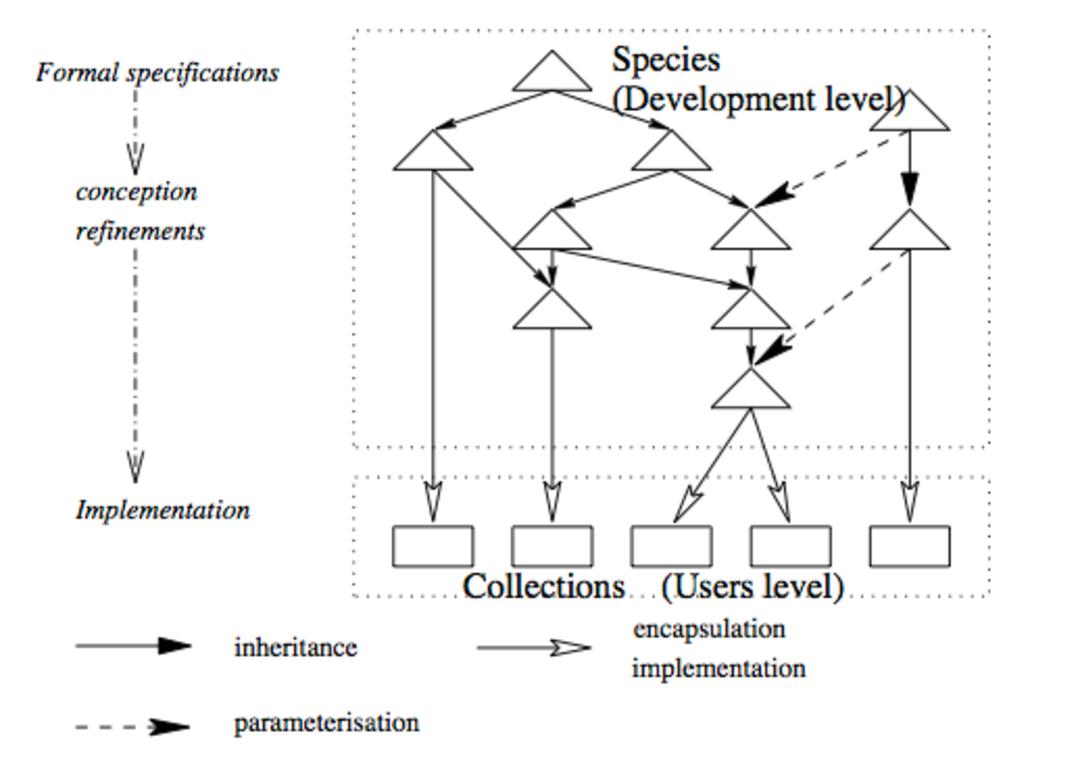
\includegraphics[width=9cm]{GFocal.pdf}
    \caption{\focalize}
    \label{fig:focal}
  \end{center}
\end{figure}

The main (object-oriented) features of \focalize are illustrated in
Figure~\ref{fig:focal}: a \focalize development is organized as a
hierarchy which may have several roots.
The upper levels of the hierarchy are built during the specification
stage while the lower ones correspond to implementations.

\paragraph{Inheritance}
Using inheritance in \focalize, one can
enrich a species with additional operations (methods) and
redefine some methods of the parent species, but one can also get
closer to a runnable implementation by providing explicit definitions to methods
that were only declared in the parent.
Note that the inheritance framework requires to perform static analysis in order
to check coherence properties (inheritance lookup, resolution of 
multiple-inheritance conflicts, dependency analysis, type-checking,
etc).
In \focalize, classical object-oriented features have been restricted
in order to
avoid unsound constructions that can lead to inconsistencies when used
carelessly.
A species can
inherit the declarations and definitions of one or several already
defined species and is
free to define or
redefine any inherited method as long as such (re)definition does not
change the type of the method.

\paragraph{Collections}

A collection is built upon a completely defined species. This means
that every method must be defined. In other words, in a collection, every 
operation has an implementation, and every theorem is formally proved.
In addition, a collection is ``frozen'': it cannot be used as a parent
of a species in the inheritance graph. Moreover, to ensure modularity
and abstraction, the carrier of a collection is hidden: seen from the
outside, it becomes an abstract type. This means
that any software component dealing with a collection will only be
able to manipulate it through the operations it
provides (i.e. its methods). This point is especially important since
it prevents other
software components from breaking representation invariants required by the
internals of the collection.

\paragraph{Parameterization}

Besides inheritance, another important feature of \focalize is the ability to
parameterize a species by generic collections instanciating a species. Such a
mechanism allows to use a species, not to embed its methods, but rather to
use it as an ``ingredient'' to build a new structure by calling its methods
explicitly.




\section{The example of binary relations}

\subsection{Definitions as Properties}

\subsubsection{Building formal specifications {\it versus} Understanding
  mathematical definitions as properties}

from absrtact binary relation to bijections

(multi)-heritage, parameterization


Ex: We define $k$ as an object such that $P(k)$.

\subsubsection{Formal reasoning on specifications {\it versus} Deducing
  properties from properties}

Ex: An object such that $P_1, \cdots, P_n$ is such that $P$.

composition de relation + quelles proprietes  ? 

preuve sur des specs

\subsection{Definitions as Computations}

\subsubsection{Programs {\it versus} Constructive definitions}

Ex: We define $k$ as obtained by $f(p)$

\subsubsection{Certified programming {\it versus} Deducing properties
  over computations}

implantation + preuves sur des implantations

Ex: $f(p)$ is such that ...

rajouter la species avec la fonction en param et qui definit la
relation avec les props. (cf LTS)


\section{Conclusion}

interet d'utiliser un outil logiciel dans l'enseignement ...
We think that \focalize is a good candidate to mix both formal
methods and discrete mathematics courses. Indeed,  \focalize provides
a formal integrated development environment simple enough to be 
usable by most students at university, even if they are not fully
acquainted with theoretical concepts (such as 
higher-order logics), in particular by making development
of proofs as easy as possible and as readable  as possible.

\paragraph{Acknowledgments}
The authors would like to thank B\'eatrice B\'erard, Damien Doligez, Th\'er\`ese Hardin,
Fran\c{c}ois Pessaux,  and Renaud Rioboo for enlightening discussions
about teaching formal methods and discrete mathematics.



%\nocite{*}
\bibliographystyle{eptcs}
\bibliography{fbibli}
\end{document}
